\documentclass{beamer}

\usepackage[utf8]{inputenc}
\usepackage[T1]{fontenc}
\usepackage[english]{babel}
\usepackage{tikz}

\usetheme{default}

\newcommand{\bigO}[1]{\mathcal O \left( #1\right)}


\title{MPRI 2.19 - Programming project}
\subtitle{Analysis of cyclic attractors for \\ asynchronous boolean models of cellular networks}
\author{Marc Heinrich \and Baptiste Lefebvre}
\institute{École Normale Supérieure, Computer Science Department}
\date{February 24, 2015}


% README
% 
% Soutenance mardi 24 février entre 09h30 et 11h30.
% 
% Objectif:
%   - présenter le projet de programmation
%   - présenter qui a fait quoi pour la réalisation du projet
%   - présenter les résultats obtenus
%
% Durée:
%   - 25 minutes de présentation
%   - 15 minutes de questions


\begin{document}


\section*{Title}

\begin{frame}
  \titlepage
\end{frame}


\section*{Table of contents}

\begin{frame}
  \frametitle{Table of contents}
  \tableofcontents
\end{frame} 


% Presentation %%%%%%%%%%%%%%%%%%%%%%%%%%%%%%%%%%%%%%%%%%%%%%%%%%%%%%%%%%%%%%%%%

\section{Presentation}

\begin{frame}
  \frametitle{Presentation}    
  %Implementation of algorthms integrated in GINsim
  TODO: complete
  
  TEST: cite \cite{Bonzanni}
\end{frame}

\begin{frame}
\begin{figure}
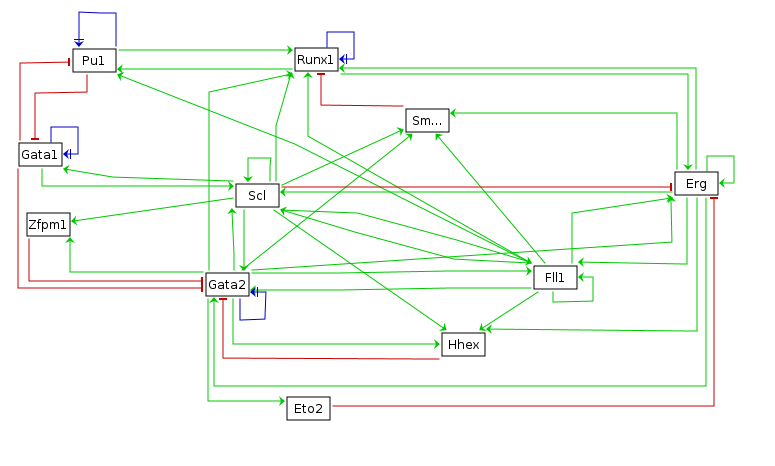
\includegraphics[scale=0.4]{hematopoietic}
\caption{Boolean Model for blood stem cells}
\end{figure}

\end{frame}

\subsection{Introduction to MDDs}
%Maybe not put here
%Slides from previous presentation
\begin{frame}
% 2 minutes
\frametitle{BDDs/MDDs}
Représentation compacte d'une fonction booléenne à $n$ variables.
\begin{figure}
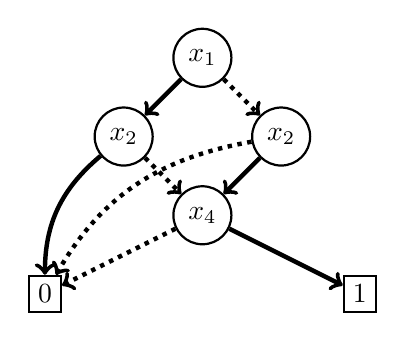
\begin{tikzpicture}
\tikzstyle{endnode} = [draw, rectangle, thick, black] ;
\tikzstyle{varnode} = [draw, circle, thick, black] ;
\tikzstyle{onearrow} = [->, ultra thick, black] ;
\tikzstyle{zeroarrow} = [->, ultra thick, black, dotted] ;
\node[varnode] (x1) at (0,0) {$x_1$} ;
\node[varnode] (1x2) at (-1,-1) {$x_2$} ;
\node[varnode] (2x2) at (1,-1) {$x_2$} ;
\node[varnode] (x4) at (0,-2) {$x_4$} ;
\node[endnode] (1) at (2,-3) {1} ; 
\node[endnode] (0) at (-2,-3) {0} ;
\draw[onearrow] (x1) -- (1x2) ;
\draw[onearrow] (1x2) to[out=-140, in=90] (0) ;
\draw[onearrow] (x4) -- (1) ;
\draw[onearrow] (2x2) -- (x4) ;
\draw[zeroarrow] (x1) -- (2x2) ;
\draw[zeroarrow] (2x2) to[out=-170, in = 60] (0) ;
\draw[zeroarrow] (1x2) -- (x4) ;
\draw[zeroarrow] (x4) -- (0) ;
\end{tikzpicture}
\end{figure}

\begin{definition}
MDD : Extension to multivalued variables
\end{definition}

\end{frame}

\begin{frame}
\frametitle{Operations on MDDs}
\begin{itemize}
\item Apply binary operators (ex: AND, OR, EQUAL, ....)

\bigskip
\item Apply existential/universal quantifiers

\bigskip
\item Substitute variables

\bigskip
\item Composition of functions

\bigskip
\item Find satisfying assignments
\end{itemize}
\end{frame}

\begin{frame}
%Mettre l'intérêt de cette structure de données

\begin{block}{Pros}
\begin{itemize}
\item Compact representation of Boolean/Integer functions
\item Represent a set of states by its indicator function.
\end{itemize}
\end{block}

\bigskip
\begin{block}{Cons}
\begin{itemize}
\item De taille potentiellement exponentielle
\item La taille dépend de l'ordre des variables
\end{itemize}
\end{block}
\end{frame}

% Distribution of tasks %%%%%%%%%%%%%%%%%%%%%%%%%%%%%%%%%%%%%%%%%%%%%%%%%%%%%%%%

\section{Distribution of tasks}

\begin{frame}
% 1 minute
  \frametitle{Distribution of tasks}
  TODO: complete
- Finding minimum perturbation
- MDD based algorithm for attractors
- LIP based algorithm  
  
\end{frame}

\begin{frame}
% 2- minutes
	\frametitle{Finding the minimum perturbation}
	TODO: explain problem
	TODO: explain example Bonzanni
	TODO: explain simple solution
	TODO: idea of improvement
\end{frame}

\begin{frame}
% 3-4 minutes
	\frametitle{Finding attractors}
	TODO: describe Garg Algorithm (pseudo-code)
	TODO: synchrone and asynchrone
	TODO: idea of improvement
\end{frame}

\begin{frame}
% Bapt : LIP based algo
	TODO 

\end{frame}


% Results %%%%%%%%%%%%%%%%%%%%%%%%%%%%%%%%%%%%%%%%%%%%%%%%%%%%%%%%%%%%%%%%%%%%%%

\section{Results}

\begin{frame}
  \frametitle{Results}
  %Demonstration on GINsim of the different plugins?   
  TODO: complete
\end{frame}


\section*{References}

\begin{frame}
  \frametitle{References}
  \bibliographystyle{apalike}
  \bibliography{presentation.bib}
\end{frame}


\end{document}
